\setcounter{section}{31}
\setcounter{ex}{0}
\section{Xét tính đơn điệu của hàm số}
\subsection{Kiến thức cần nhớ}
\begin{khung}
	\subsubsection{Định nghĩa}
	\begin{itemize}
		\item Hàm số $y=f(x)$ được gọi là đồng biến (tăng) trên $\mathscr{K}$ khi $f'(x)\geq 0\, \forall x\in \mathscr{K}$.
		\item Hàm số $y=f(x)$ được gọi là nghịch biến (giảm) trên $\mathscr{K}$ khi $f'(x)\leq 0\, \forall x\in \mathscr{K}$.
	\end{itemize}
	\subsubsection{Các bước thực hiện khi xét tính đơn điệu của hàm số}
	\begin{itemize}
		\item {\bfseries Bước 1.} Tính $y'=f'(x)$. Cho $f'(x)=0$ tìm nghiệm (nếu có).
		\item {\bfseries Bước 2.} Lập bảng biến thiên của hàm số.
		\item {\bfseries Bước 3.} Dựa vào bảng biến thiên, kết luận miền đơn điệu của hàm số.
	\end{itemize}
\end{khung}
\subsection{Bài tập mẫu}
\Opensolutionfile{ans}[ans/ANS-DANG-32]
\begin{khung}
\begin{vd}[Đề tham khảo BGD 2022-2023]%[Trần Tú]%[2D1B1-1]%Câu 26
	Cho hàm số $f(x)$ có đạo hàm $f'(x)=\left(x+1\right)^2\left(x-1\right)^3\left(2-x\right)$. Hàm số $f(x)$ đồng biến trên khoảng nào dưới đây?
	\choice
	{$\left(-1; 1\right)$}
	{$\left(2; +\infty\right)$}
	{\True $\left(1; 2\right)$}
	{$\left(-\infty; -1\right)$}
\loigiai{
	Ta có $f'(x)=0\Leftrightarrow x\in \{-1; 1; 2\}$. Ta có bảng biên thiên như sau
	\begin{center}
		\begin{tikzpicture}
			\tkzTab[lgt=1.3,espcl=2] % tùy chọn
			{$x$/.8, $f’(x)$/.8, $f(x)$/1.5} % cột đầu tiên
			{$-\infty$, $-1$, $1$, $2$, $+\infty$ } % hàng 1 cột 2
			{,-,0,-,0,+,0,-,} % hàng 2 cột 2
			{+/, R/,-/, +/,-/} % hàng 3 cột 2
			%\tkzTabIma{1}{3}{2}{} % hàng 3 cột 2 (điểm giữa)
		\end{tikzpicture}
	\end{center}
	Từ bảng biến thiên ta thấy hàm số đồng biến trên khoảng $\left(1; 2\right)$.
}
\end{vd}
\end{khung}
\subsection{Bài tập tương tự và phát triển}
\begin{ex}%[Trần Tú]%[2D1B1-1]
	Cho hàm số$ f(x)$ có đạo hàm$f'(x)=x\left(x-1\right)^3\,\,\forall x\in \mathbb{R}$ nghịch biến trên khoảng nào?
	\choice
	{$\left(-\infty; 0\right)$}
	{$\left(-1; 1\right)$}
	{\True $\left(0; 1\right)$}
	{$\left(1; +\infty\right)$}
\loigiai{
	Bảng xét dấu của $f'(x)$.
	\begin{center}
\begin{tikzpicture}
\tkzTabInit[lgt=1.2,espcl=3]
{$x$ /0.6, $f’(x)$ /0.6, $f(x)$ /2}
{$-\infty$,$x_1$,$x_2$,$+\infty$}
\tkzTabLine{ ,+,$0$,-,$0$,+, }
\tkzTabVar{-/,+/,-/,+/}
\end{tikzpicture}
\end{center}
	Từ bảng biến thiên, ta thấy hàm số nghịch biến trên $(0; 1)$.
}
\end{ex}

\begin{ex}%[Trần Tú]%[2D1B1-1]
	Cho hàm số $y=f(x)$ có đạo hàm $f'(x)=x^2+1$. Khẳng định nào sau đây đúng?
	\choice
	{Hàm số nghịch biến trên $\left(-\infty; +\infty\right)$}
	{Hàm số nghịch biến trên $\left(-1; 1\right)$}
	{\True Hàm số đồng biến trên $\left(-\infty; +\infty\right)$}
	{Hàm số nghịch biến trên $\left(-\infty; 1\right)$}
\loigiai{
	Ta có $ f'(x)=x^2+1>0,\forall x\in \mathbb{R}$ do vậy hàm số đồng biến trên $\left(-\infty; +\infty\right)$.
}
\end{ex}

\begin{ex}%[Trần Tú]%[2D1B1-1]
	Cho hàm số $y=f(x)$có đạo hàm liên tục trên $\mathbb{R}$ và $y=f'(x)<0\,\, \forall x\in\left(-3; 5\right)$. Khẳng định nào sau đây đúng?
	\choice
	{$f(0)<f(5)$}
	{\True $f\left(-3\right)>f(5)$}
	{$f\left(-3\right)<f(5)$}
	{$f\left(-2\right)=f(2)$}
\loigiai{
	Dễ thấy hàm số nghịch biến trên đoạn $\left[-3; 5\right]$ và $-3<5$ nên suy ra $f\left(-3\right)>f(5)$.
}
\end{ex}

\begin{ex}%[Trần Tú]%[2D1B1-1]
	Hàm số $f(x)$ có $f'(x)=\left(x-1\right)\left(x-2\right),\forall x\in \mathbb{R}$ nghịch biến trên khoảng nào dưới đây?
	\choice
	{$\left(2; +\infty\right)$}
	{$\left(-\infty; -1\right)$}
	{$\left(-2; -1\right)$}
	{\True $\left(1; 2\right)$}
\loigiai{
	Ta có $f'(x)<0 \Leftrightarrow \left(x-1\right)\left(x-2\right)<0
	\Leftrightarrow 1<x<2$.
}
\end{ex}

\begin{ex}%[Trần Tú]%[2D1B1-1]
	Cho hàm số $y=f(x)$ có đạo hàm $f'(x)=\left(x^2-1\right)\left(x+1\right)\left(5-x\right)$. Mệnh đề nào sau đây đúng?
	\choice
	{$ f(2)<f(1)<f(4)$}
	{$ f(4)<f(2)<f(1)$}
	{$ f(1)<f(4)<f(2)$}
	{\True $ f(1)<f(2)<f(4)$}
\loigiai{
	Ta có $f'(x)=\left(x^2-1\right)\left(x+1\right)\left(5-x\right)=0\Leftrightarrow x=\pm 1,x=5$. Xét bảng biến thiên
	\begin{center}
		\begin{tikzpicture}
			\tkzTab[lgt=1.3,espcl=2] % tùy chọn
			{$x$/0.6, $f’(x)$/0.6, $f(x)$/2} % cột đầu tiên
			{$-\infty$, $-1$, $1$, $5$ , $+\infty$ } % hàng 1 cột 2
			{,-,0,-,0,+,0,-,} % hàng 2 cột 2
			{+/, R/,-/ , +/, -/} % hàng 3 cột 2
			%\tkzTabIma{1}{3}{2}{}
		\end{tikzpicture}
	\end{center}
	Dựa vào bảng biến thiên ta có $f(1)<f(2)<f(4)$.}
\end{ex}

\begin{ex}%[Trần Tú]%[2D1B1-1]
	Cho hàm số $y=f(x)$ liên tục trên $\mathbb{R}$ và có đạo hàm $f'(x)=\left(x+1\right)^2\left(x-1\right)^3\left(2-x\right)$. Hàm số $y=f(x)$ đồng biến trên khoảng nào dưới đây?
	\choice
	{$\left(2; +\infty\right)$}
	{$\left(-\infty; -1\right)$}
	{$\left(-1; 1\right)$}
	{\True $\left(1; 2\right)$}
\loigiai{
	Ta có $f'(x)=0\Leftrightarrow \left(x+1\right)^2\left(x-1\right)^3\left(2-x\right)=0
	\Leftrightarrow \hoac{& x=-1\\ & x=1\\ & x=2.}$\\
	Lập bảng xét dấu của $f'(x)$ ta được:
	\begin{center}
		\begin{tikzpicture}
			\tkzTab[lgt=1.3,espcl=2] % tùy chọn
			{$x$/0.6, $f’(x)$/0.6, $f(x)$/2} % cột đầu tiên
			{$-\infty$, $-1$, $1$,$2$, $+\infty$ } % hàng 1 cột 2
			{,-,0,-,0,+,0,-,} % hàng 2 cột 2
			{+/, R/ , -/, +/,-/} % hàng 3 cột 2
			%\tkzTabIma{1}{3}{2}{}
		\end{tikzpicture}
	\end{center}
	Vậy hàm số $ y=f(x)$ đồng biến trên khoảng $\left(1; 2\right)$.
}
\end{ex}

\begin{ex}%[Trần Tú]%[2D1B1-1]
	Cho hàm số $ y=f(x)$ có đạo hàm trên $\mathbb{R}$ là $f'(x)=x^2(x-1)$. Hàm số $y=f(x)$ đồng biến trên khoảng nào sau đây?
	\choice
	{$\left(-\infty; \,+\infty\right)$}
	{\True $\left(1; \,+\infty\right)$}
	{$\left(-\infty; \,1\right)$}
	{$\left(0; \,1\right)$}
\loigiai{
	Ta có $f'(x)=x^2(x-1)>0,\,\forall\,x>1$ nên hàm số đồng biến trên khoảng $\left(1; \,+\infty\right)$.
}
\end{ex}

\begin{ex}%[Trần Tú]%[2D1B1-1]
	Cho hàm số $y=f(x)$có đạo hàm $f'(x)=x{\left(x-2\right)^3}$, với mọi $x\in \mathbb{R}$. Hàm số đã cho nghịch biến trên khoảng nào dưới đây?
	\choice
	{\True $\left(0; 1\right)$}
	{$\left(-2; 0\right)$}
	{$\left(1; 3\right)$}
	{$\left(-1; 0\right)$}
\loigiai{
	Ta có $f'(x)=0 \Leftrightarrow \hoac{& x=0\\ & x=2.}$\\
	Đồng thời $f'(x)<0 \Leftrightarrow x\in\left(0; 2\right)$ nên ta chọn đáp án theo đề bài là $\left(0; 1\right)$.
}
\end{ex}

\begin{ex}%[Trần Tú]%[2D1B1-1]
	Hàm số $y=f(x)$có đạo hàm $y'=x^2$. Mệnh đề nào sau đây đúng?
	\choice
	{Hàm số nghịch biến trên $\left(-\infty; 0\right)$và đồng biến trên $\left(0; +\infty\right)$}
	{\True Hàm số đồng biến trên $\mathbb{R}$}
	{Hàm số đồng biến trên $\left(-\infty; 0\right)$và nghịch biến trên $\left(0; +\infty\right)$}
	{Hàm số nghịch biến trên $\mathbb{R}$}
\loigiai{
	Ta có $y'=x^2 \,\, x\in \mathbb{R}$. Vậy hàm số đồng biến trên $\mathbb{R}$.
}
\end{ex}

\begin{ex}%[Trần Tú]%[2D1B1-1]
	Hàm số $y=f(x)$ có đạo hàm $f'(x)=x^2+1$. Khẳng định nào sau đây đúng?
	\choice
	{Hàm số nghịch biến trên $(-\infty; +\infty)$}
	{Hàm số nghịch biến trên $(-1; 1)$}
	{\True Hàm số đồng biến trên $(-\infty; +\infty)$}
	{Hàm số nghịch biến trên $(-\infty; 1)$}
\loigiai{
	Ta có $f'(x)=x^2+1>0 \,\, \forall x\in \mathbb{R}$ nên hàm số $y=f(x)$ đồng biến trên $(-\infty; +\infty)$.
}
\end{ex}

\begin{ex}%[Trần Tú]%[2D1B1-1]
	Cho hàm số $y=f(x)$ có đạo hàm $f'(x)=x^2+1$, $\forall x\in \mathbb{R}$. Mệnh đề nào dưới đây đúng?
	\choice
	{Hàm số nghịch biến trên khoảng $\left(-1; 1\right)$}
	{\True Hàm số đồng biến trên khoảng $\left(-\infty; +\infty\right)$}
	{Hàm số nghịch biến trên khoảng $\left(-\infty; 0\right)$}
	{Hàm số nghịch biến trên khoảng $\left(1; +\infty\right)$}
\loigiai{
	Do hàm số $y=f(x)$ có đạo hàm $f'(x)=x^2+1>0\,\, \forall x\in \mathbb{R}$ nên hàm số đồng biến trên khoảng $\left(-\infty; +\infty\right)$.
}
\end{ex}

\begin{ex}%[Trần Tú]%[2D1B1-1]
	Cho hàm số $y=f(x)$ có đạp hàm $f'(x)=x^2+1\,\, \forall x\in \mathbb{R}$. Mệnh đề nào dưới đây đúng?
	\choice
	{Hàm số nghịch biến trên khoảng $\left(-1; 1\right)$}
	{\True Hàm số đồng biến trên khoảng $\left(-\infty; +\infty\right)$}
	{Hàm số nghịch biến trên khoảng $\left(-\infty; 0\right)$}
	{Hàm số nghịch biến trên khoảng $\left(1; +\infty \right)$}
\loigiai{
	Ta có $f'(x)=x^2+1>0\,\, \forall x\in \mathbb{R} \Rightarrow$ hàm số đồng biến trên khoảng $\left(-\infty; +\infty\right)$.
}
\end{ex}

\begin{ex}%[Trần Tú]%[2D1B1-1]
	Hàm số $ f(x)$liên tục trên $\mathbb{R}$và có đạo hàm $f'(x)=x^2+4$ với mọi $x\in \mathbb{R}$. Khẳng định nào sau đây là đúng về sự biến thiên của hàm số $f(x)$?
	\choice
	{\True $f(x)$ đồng biến trên $\mathbb{R}$}
	{$f(x)$ chỉ đồng biến trên khoảng $\left(-2; 2\right)$ trong tập $\mathbb{R}$}
	{$f(x)$ nghịch biến trên $\mathbb{R}$}
	{$ f(x)$ chỉ nghịch biến trên khoảng $\left(-2; 2\right)$ trong tập $\mathbb{R}$}
\loigiai{
	Ta có hàm số $f(x)$ liên tục trên $\mathbb{R}$ và có đạo hàm $f'(x)=x^2+4>0$ với mọi $x\in \mathbb{R}$.\\
	Do đó hàm số $f(x)$ đồng biến trên $\mathbb{R}$.
}
\end{ex}

\begin{ex}%[Trần Tú]%[2D1B1-1]
	Cho hàm số $ y=f(x)$có $f'(x)=\left(x+2\right)\left(x+1\right)\left(x^2-1\right)$. Hàm số $y=f(x)$ đồng biến trên khoảng nào sau đây?
	\choice
	{$\left(-2; -1\right)$}
	{$\left(-1; 1\right)$}
	{\True $\left(0; +\infty\right)$}
	{$\left(-\infty; -2\right)$}
\loigiai{
	Ta có $f'(x)=\left(x+2\right)\left(x+1\right)\left(x^2-1\right)
	=\left(x+2\right)\left(x-1\right)\left(x+1\right)^2$.\\
	Cho $f'(x)=0\Leftrightarrow \hoac{& x=-2\\ & x=-1\\ & x=1}$. 
	Bảng biến thiên
	\begin{center}
		\begin{tikzpicture}
			\tkzTab[lgt=1.3,espcl=2] % tùy chọn
			{$x$/0.6, $f’(x)$/0.6, $f(x)$/2} % cột đầu tiên
			{$-\infty$, $-2$, $-1$, $1$ , $+\infty$ } % hàng 1 cột 2
			{,+,0,-,0,-,0,+,} % hàng 2 cột 2
			{-/, +/, R/ , -/, +/} % hàng 3 cột 2
			%\tkzTabIma{2}{4}{3}{}
		\end{tikzpicture}
	\end{center}
}
\end{ex}

\begin{ex}%[Trần Tú]%[2D1B1-1]
	Hàm số $f(x)$có đạo hàm $f'(x)>0\,\, \forall x\in \mathbb{R}$. Khi đó hàm số đã cho
	\choice
	{\True đồng biến trên $\mathbb{R}$}
	{nghịch biến trên $\mathbb{R}$}
	{là hàm hằng trên $\mathbb{R}$}
	{đồng biến trên $\left(-\infty; 0\right)$ và nghịch biến trên $\left(0; +\infty\right)$}
\loigiai{
	Vì $ f'(x)>0\,\, \forall x\in \mathbb{R}$ nên hàm số $ f(x)$ đồng biến trên $\mathbb{R}$.
}
\end{ex}

\begin{ex}%[Trần Tú]%[2D1B1-1]
	Cho hàm số $ y=f(x)$ liên tục trên $\mathbb{R}$ và có đạo hàm $f'(x)=\left(1-x\right)^2\left(x+1\right)^3\left(3-x\right)$. Hàm số $y=f(x)$ đồng biến trên khoảng nào dưới đây?
	\choice
	{$\left(-\infty; \,-1\right)$}
	{\True $\left(1; \,3\right)$}
	{$\left(3; \,+\infty\right)$}
	{$\left(-\infty; \,1\right)$}
\loigiai{
	Ta có $f'(x)=0\Leftrightarrow \left(1-x\right)^2\left(x+1\right)^3\left(3-x\right)=0
	\Leftrightarrow \hoac{&x=1 \\ &x=-1\\ &x=3}$.
	Bảng biến thiên của hàm số
	\begin{center}
		\begin{tikzpicture}
			\tkzTab[lgt=1.3,espcl=2] % tùy chọn
			{$x$/0.6, $f’(x)$/0.6, $f(x)$/2} % cột đầu tiên
			{$-\infty$, $-1$, $1$ ,$3$ , $+\infty$ } % hàng 1 cột 2
			{,-,0,+,0,+,0,-,} % hàng 2 cột 2
			{+/, -/, R/ , +/, -/} % hàng 3 cột 2
		\end{tikzpicture}
	\end{center}
	Hàm số đồng biến trên các khoảng $\left(-1; 3\right)$.
}
\end{ex}

\begin{ex}%[Trần Tú]%[2D1B1-1]
	Cho hàm số $ f(x)$ có đạo hàm là $f'(x)=x\left(x+1\right)^2$. Hàm số đồng biến trên khoảng nào dưới đây?
	\choice
	{\True $\left(0; +\infty\right)$}
	{$\left(-1; 0\right)$}
	{$\left(-\infty; -1\right)$}
	{$\left(-1; +\infty\right)$}
\loigiai{
	Ta có $ f'(x)=0\Leftrightarrow \hoac{& x=0\\ & x=-1}$. Bảng biến thiên
	\begin{center}
		\begin{tikzpicture}
			\tkzTab[lgt=1.3,espcl=2] % tùy chọn
			{$x$/0.6, $f’(x)$/0.6, $f(x)$/2} % cột đầu tiên
			{$-\infty$, $-1$, $0$ , $+\infty$ } % hàng 1 cột 2
			{,-,0,-,0,+,} % hàng 2 cột 2
			{+/, R/, -/ , +/} % hàng 3 cột 2
		\end{tikzpicture}
	\end{center}
	Từ bảng biến thiên ta thấy hàm số $f(x)$ đồng biến trên $\left(0; +\infty\right)$.
}
\end{ex}

\begin{ex}%[Trần Tú]%[2D1B1-1]
	Cho hàm số $y=f(x)$ liên tục trên $\mathbb{R}$ và có đạo hàm $f'(x)=\left(x+1\right)^2\left(x-1\right)^3\left(2-x\right)$. Hàm số $y=f(x)$ đồng biến trên khoảng nào dưới đây?
	\choice
	{$\left(-1; 1\right)$}
	{$\left(2; +\infty\right)$}
	{\True $\left(1; 2\right)$}
	{$\left(-\infty; -1\right)$}
\loigiai{
	Bảng biến thiên
	\begin{center}
		\begin{tikzpicture}
			\tkzTab[lgt=1.3,espcl=2] % tùy chọn
			{$x$/0.6, $f’(x)$/0.6, $f(x)$/2} % cột đầu tiên
			{$-\infty$, $-1$, $1$ ,$2$ , $+\infty$ } % hàng 1 cột 2
			{,-,0,-,0,+,0,-,} % hàng 2 cột 2
			{+/, R/, -/ , +/, -/} % hàng 3 cột 2
		\end{tikzpicture}
	\end{center}
	Dựa vào bảng xét dấu ta thấy hàm số đồng biến trên khoảng $\left(1; 2\right)$.
}
\end{ex}

\begin{ex}%[Trần Tú]%[2D1B1-1]
	Cho hàm số $ y=f(x)$ có đạo hàm $f'(x)=\left(x-1\right)^2,\forall x\in \mathbb{R}$. Mệnh đề nào dưới đây là sai?
	\choice
	{Hàm số đồng biến trên khoảng $\left(1\,; +\infty\right)$}
	{Hàm số đồng biến trên khoảng $\left(-\infty; +\infty\right)$}
	{\True Hàm số nghịch biến trên khoảng $\left(-\infty; 1\right)$}
	{Hàm số đồng biến trên khoảng $\left(-\infty\,; 1\right)$}
\loigiai{
	Do $f'(x)=\left(x-1\right)^2\ge 0,\forall x\in \mathbb{R}$ nên hàm số $y=f(x)$ đồng biến trên $\mathbb{R}$.
}
\end{ex}

\begin{ex}%[Trần Tú]%[2D1B1-1]
	Cho hàm số $y=f(x)$ liên tục trên $\mathbb{R}$, có đạo hàm $f'(x)=\left(x-2\right)^4+1$. Khẳng định nào sau đây đúng?
	\choice
	{\True Hàm số $y=f(x)$ đồng biến trên khoảng $\left(2; +\infty\right)$ và nghịch biến trên khoảng $\left(-\infty; 2\right)$}
	{Hàm số $y=f(x)$ đồng biến trên khoảng $\left(-\infty; +\infty\right)$}
	{Hàm số $y=f(x)$ nghịch biến trên khoảng $\left(-\infty; +\infty\right)$}
	{Hàm số $y=f(x)$ đồng biến trên khoảng $\left(-\infty; 2\right)$ và nghịch biến trên khoảng $\left(2; +\infty\right)$}
\loigiai{
	Ta có $f'(x)=\left(x-2\right)^4+1>0,\,\,\forall x\in \mathbb{R}$. Suy ra hàm số đồng biến trên $\mathbb{R}$.
}
\end{ex}

%\begin{ex}
%	Cho hàm số $ y=f(x)$ có đạo hàm xác định trên $\mathbb{R}$ và có biểu thức đạo hàm $f'(x)=\left(x+1\right)\left(x-3\right)$. Hàm số $y=f\left(2x+3\right)$ nghịch biến trên khoảng nào dưới đây?
%	\choice
%	{$\left(-3; -1\right)$}
%	{$\left(0; 1\right)$}
%	{$\left(1; 2\right)$}
%	{\True $\left(-1; 0\right)$}
%	\loigiai{
%		Ta có\\
%		Xét hàm số $g(x)=f\left(2x+3\right)\Rightarrow g'(x)=2f'\left(2x+3\right)=2.\left(2x+4\right)\left(2x\right)$\\
%		Lập bảng xét dấu\\
%		\\
%		Từ bảng xét dấu ta có khoảng nghịch biến của hàm số $g(x)=f\left(2x+3\right)$ là $\left(-2; 0\right)$.
%	}
%\end{ex}
%
%\begin{ex}%Câu 22
%	Hàm số $ y=f(x)$có đạo hàm $f'(x)<0,\,\,\forall x\in \mathbb{R}$. Tìm $x$ để $ f\left(\dfrac{1}{x}\right)>f(2).$
%	\choice
%	{$\left(0; \dfrac{1}{2}\right)$}
%	{$\left(-\infty; \dfrac{1}{2}\right)$}
%	{$\left(-\infty; 0\right)\cup\left(0\,; \dfrac{1}{2}\,\right)$}
%	{\True $\left(-\infty; 0\right)\cup\left(\dfrac{1}{2}; +\infty\right)$}
%	\loigiai{
%		Do hàm số $y=f(x)$ có đạo hàm $f'(x)<0,\,\,\forall x\in \mathbb{R}$ nên:\\
%		$ f\left(\dfrac{1}{x}\right)>f(2)
%		\Leftrightarrow \dfrac{1}{x}<2 
%		\Leftrightarrow \dfrac{1-2x}{x}<0
%		\Leftrightarrow x\in\left(-\infty; 0\right)\cup\left(\dfrac{1}{2}; +\infty\right)$.
%	}
%\end{ex}
%
%\begin{ex}%Câu 23
%	Cho hàm số $ y=f(x)$ có đạo hàm $f'(x)=x^2-2x$ với mọi $ x\in \mathbb{R}$. Hàm số $ g(x)=-2f(x)$ đồng biến trên khoảng
%	\choice
%	{$\left(2; \,+\infty\right)$}
%	{$\left(-\infty; \,-2\right)$}
%	{\True $\left(0; \,2\right)$}
%	{$\left(-2; \,0\right)$}
%	\loigiai{
%		Ta có $g'(x)=-2f'(x)=-2\left(x^2-2x\right)$.\\
%		$g'(x)>0\Leftrightarrow x^2-2x<0
%		\Leftrightarrow 0<x<2$. Suy ra, hàm số đồng biến trên $\left(0; \,2\right)$.
%	}
%\end{ex}
%
%\begin{ex}%Câu 24
%	Hàm số $ f(x)$có đạo hàm trên $\mathbb{R}$và $ f'(x)>0,\forall x\in\left(0; +\infty\right)$, biết $ f(2)=1$. Khẳng định nào sau đây có thể xảy ra?
%	\choice
%	{\True $f(2)+f(3)=4$}
%	{$f(1)=4$}
%	{$f\left(2019\right)>f\left(2020\right)$}
%	{$f(3)=0$}
%	\loigiai{
%		Ta có hàm số $ f(x)$có đạo hàm trên $\mathbb{R}$ và $ f'(x)>0,\forall x\in\left(0; +\infty\right)$ nên hàm số $ f(x)$ đồng biến trên $\left(0; +\infty\right)$\\
%		Lại có $f(2)=1$ mà $3>2\Rightarrow f(3)>f(2)$ nên $A$ sai\\
%		$1<2\Rightarrow f(1)<f(2)$ nên $C$ sai\\
%		$2019<2020\Rightarrow f\left(2019\right)<f\left(2020\right)$ nên $D$ sai\\
%		Xét $ B$:$f(2)+f(3)=4\Rightarrow f(3)=4-f(2)=4-1=3>f(2)$\\
%		Vậy $ B$ có thể xảy ra.
%	}
%\end{ex}
\Closesolutionfile{ans}
%======================
\subsection{Bảng đáp án}
\inputansbox{8}{ans/ANS-DANG-32}


